\textcolor{blue}{Problem 1}

7.2 Additive noise channel. Find the channel capacity of the following discrete memoryless channel:
\begin{figure}[htbp]
    \centering
	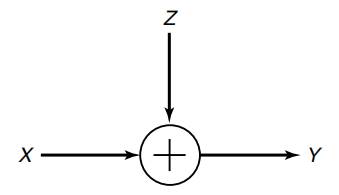
\includegraphics[width=0.35\textwidth]{../figures/7.2.png}
\end{figure}

where $\operatorname{Pr}\{Z=0\}=\operatorname{Pr}\{Z=a\}=\dfrac{1}{2}$. The alphabet for $x$ is $\mathbf{X}=$ $\{0,1\}$. Assume that $Z$ is independent of $X$. Observe that the channel capacity depends on the value of $a$.

\textcolor{blue}{Solution}

We have $\mathcal{X}=\{0,1\}, \mathcal{Z}=\{0,1\}, \mathcal{Y}=\{0,1,a,a+1\}, Y=X+Z$.

So we need to discuss the value of $a$.

<1> When $a=0$, then $P(Z=0)=P(Z=a)=\dfrac{1}{2}$, which is not a suitable probability distribution.

If we correct the probability into $P(Z=0)=1$, then we have
\begin{align*}
I(X;Y) &= H(X)-H(X|Y) \\
&= H(X) \text{\qquad (since $Y=X$, so when given $Y$, $X$ is deterministic)} \\
&\leq \log \left|\mathcal{X}\right| \\
&= 1
\end{align*}
When $p(x)=\left(\dfrac{1}{2},\dfrac{1}{2}\right)$, the inequality takes the equality. \\
So the channel capacity is $C=\max\limits_{p(x)}I(X;Y)=1$ bit.

<2> When $a=-1$, then $\mathcal{Y}= \{0,1,-1\}$, the DMC is as follows:
\begin{figure}[htbp]
    \centering
	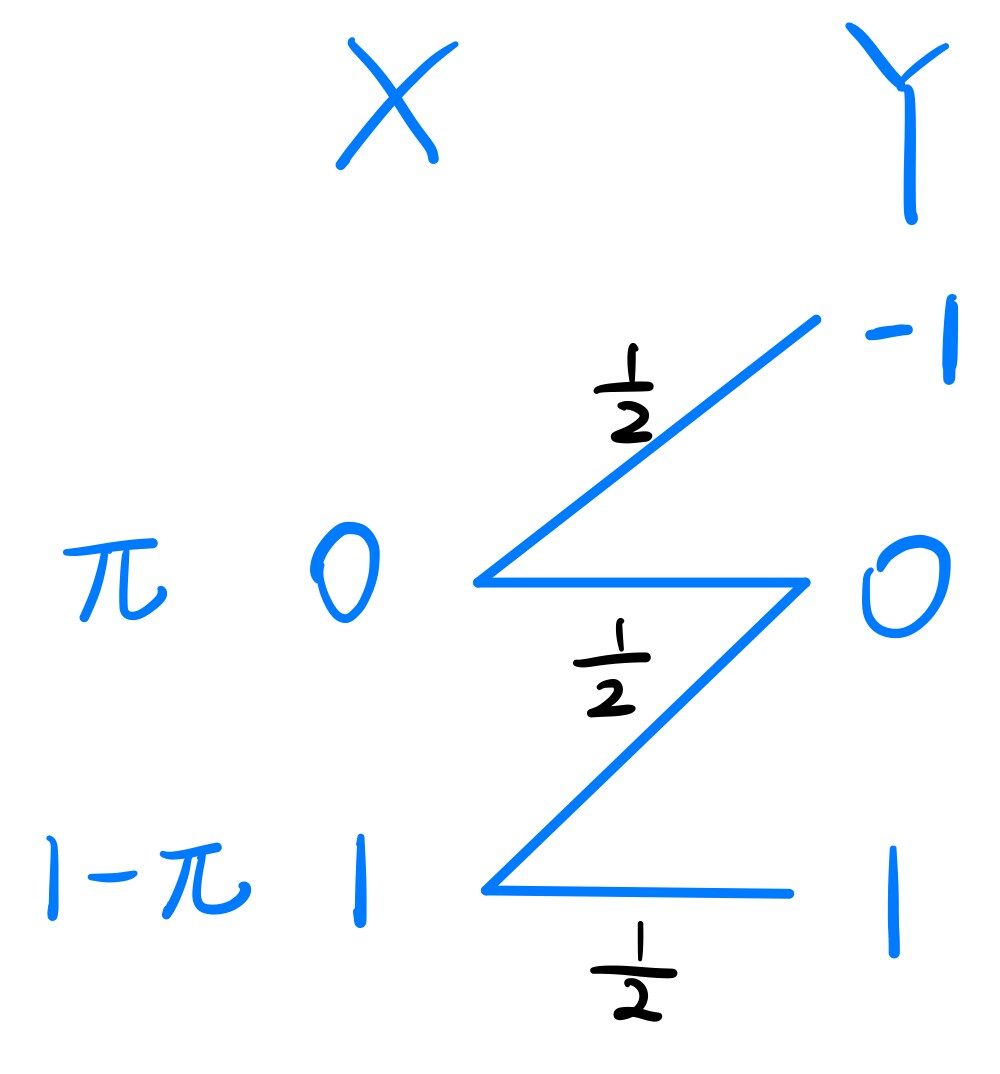
\includegraphics[width=0.35\textwidth]{../figures/7.2_-1.png}
\end{figure}

If we define $p(X=0)=\pi, p(X=1)=1-\pi$, then
$$P(Y=0) = P(Y=0|X=0)P(X=0) + P(Y=0|X=1)P(X=1) = \dfrac{1}{2}\pi + \dfrac{1}{2}(1-\pi) = \dfrac{1}{2}$$
Also, we can get that $P(X=0|Y=0)=\dfrac{P(Y=0|X=0)P(X=0)}{P(Y=0)}=\pi, P(X=1|Y=0)=1-\pi$. \\
So we have:
\begin{align*}
I(X;Y) &= H(X) - H(X|Y) \\
&= H(X) - \sum_{y}H(X|Y=y)P(Y=y) \\
&= H(X) - H(X|Y=0)p(Y=0) \qquad \text{(since when $Y=\pm 1$, $X$ is deterministic, $H(X|Y=-1)=H(X|Y=1)=0$)} \\
&= H\left(\pi,1-\pi\right) - \dfrac{1}{2}H\left(\pi,1-\pi\right) \\
&= \dfrac{1}{2}H\left(\pi,1-\pi\right) \\
&\leq \dfrac{1}{2}\log 2 = \dfrac{1}{2}
\end{align*}
If $\pi=\dfrac{1}{2}$, i.e. $p(x)=\left(\dfrac{1}{2},\dfrac{1}{2}\right)$, the inequality takes the equality. \\
So the channel capacity is $C=\max\limits_{p(x)}I(X;Y)=\dfrac{1}{2}$ bit.

<3> When $a=1$, then $\mathcal{Y}= \{0,1,2\}$, the DMC is as follows:
\begin{figure}[htbp]
    \centering
	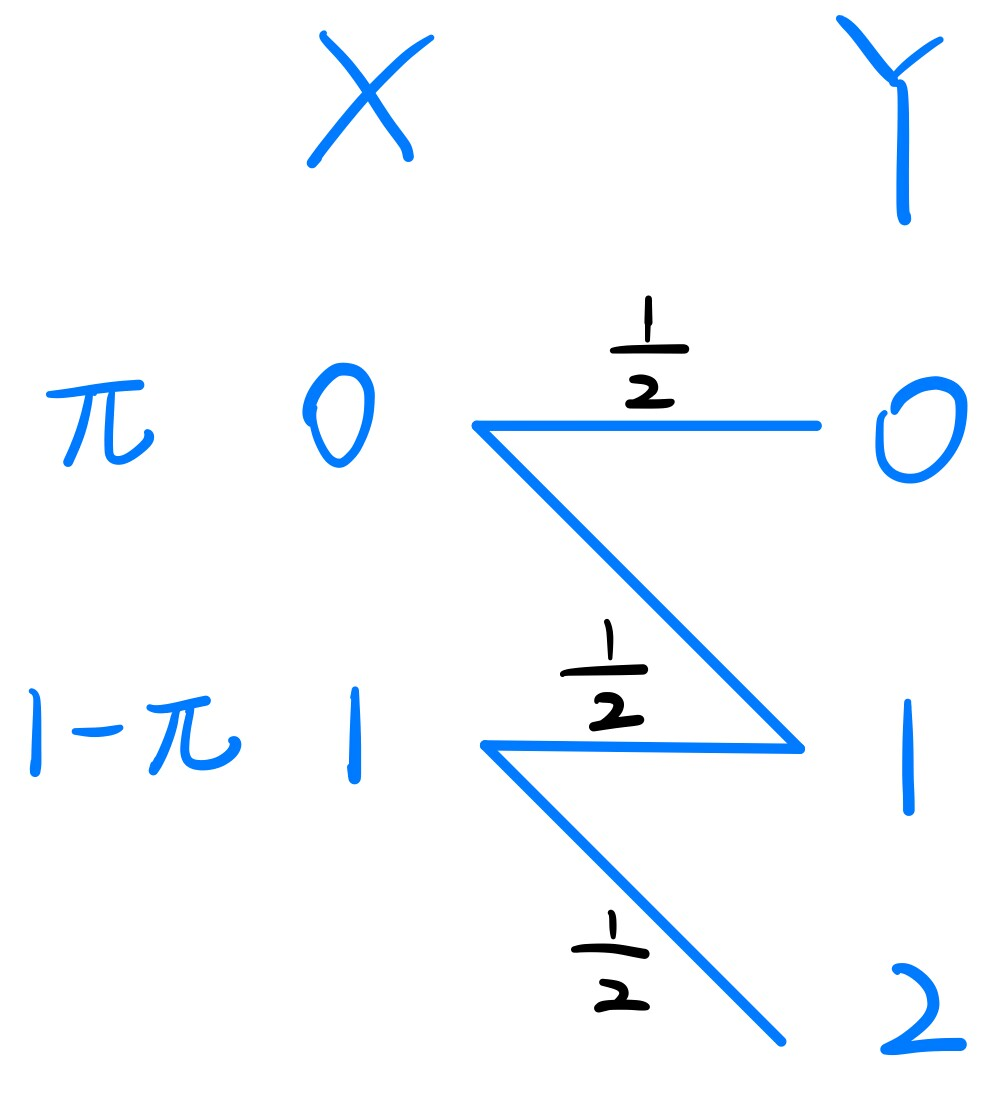
\includegraphics[width=0.35\textwidth]{../figures/7.2_1.png}
\end{figure}

Which is quite similar to the case when $a=-1$. \\
i.e. With the quite similar process, we can get that
\begin{align*}
P(Y=1) &= \dfrac{1}{2} \\
P(X=0|Y=1) &= \pi \\
I(X;Y) &= H(X) - H(X|Y) \\
&= H(X) - \sum_{y}H(X|Y=y)P(Y=y) \\
&= H(X) - H(X|Y=1)p(Y=1) \text{\ (When $Y=0,2$, $X$ is deterministic, $H(X|Y=0)=H(X|Y=2)=0$)} \\
&= H\left(\pi,1-\pi\right) - \dfrac{1}{2}H\left(\pi,1-\pi\right) \\
&= \dfrac{1}{2}H\left(\pi,1-\pi\right) \leq \dfrac{1}{2}\log 2 = \dfrac{1}{2}
\end{align*}
If $\pi=\dfrac{1}{2}$, i.e. $p(x)=\left(\dfrac{1}{2},\dfrac{1}{2}\right)$, the inequality takes the equality. \\
So the channel capacity is $C=\max\limits_{p(x)}I(X;Y)=\dfrac{1}{2}$ bit.

<4> When $a \neq 0, a \neq \pm 1$, then the channel is as follows:
\begin{figure}[htbp]
    \centering
	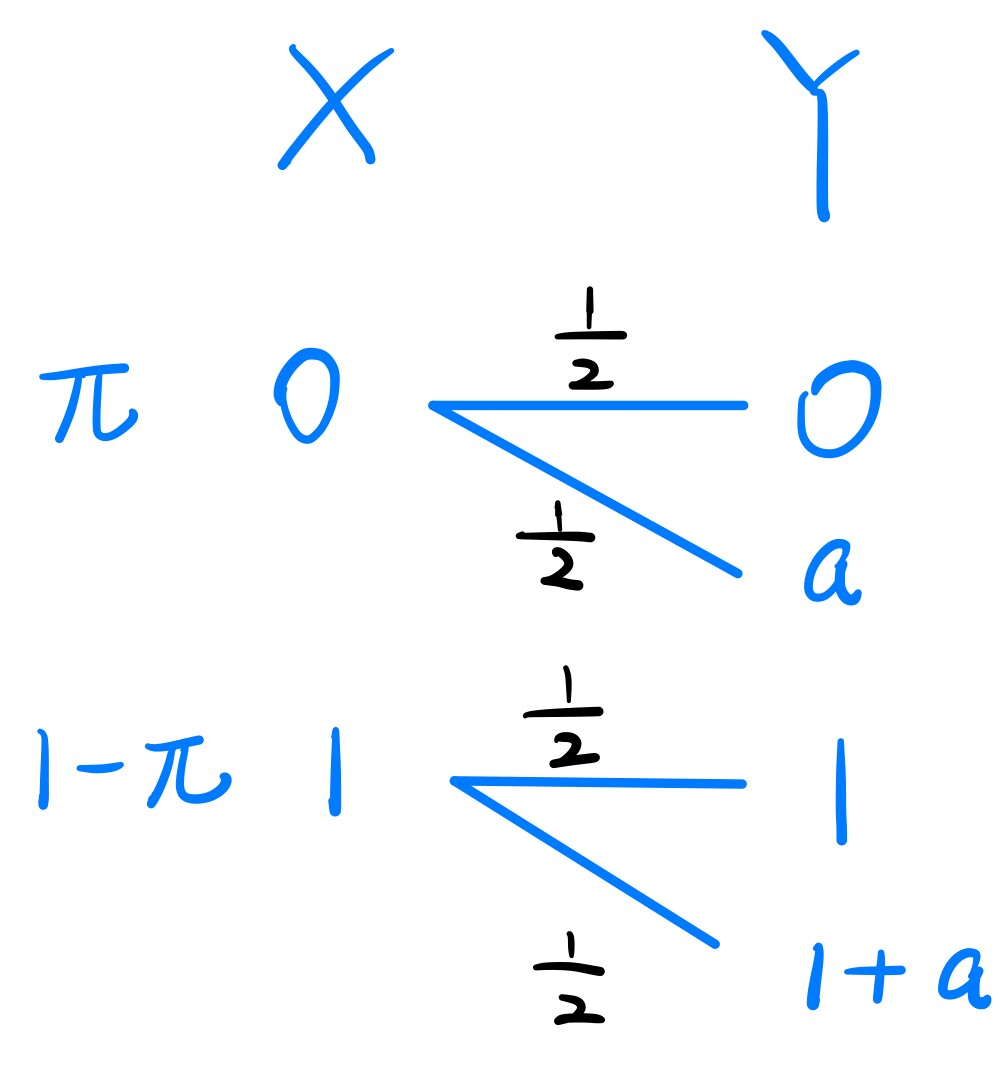
\includegraphics[width=0.35\textwidth]{../figures/7.2_otherwise.png}
\end{figure}

Which is actually a noisy channel with non-overlapping outputs.
\begin{align*}
I(X;Y) &= H(X) - H(X|Y) \\
&= H(X) \text{\qquad (When given $Y$, $X$ is deterministic)} \\
&\leq \log \left|\mathcal{X}\right| = 1
\end{align*}
So the channel capacity is $C=\max\limits_{p(x)}I(X;Y)=1$ bit.

So above all, the channel capacity of the following discrete memoryless channel is as follows:
\begin{align*}
C &= \begin{cases}
1 & \text{, if } a=0 \text{ , and the probablity is corrected into } P(X=0)=1 \\
\dfrac{1}{2} & \text{, if } a=\pm 1 \\
1 & \text{, otherwise}
\end{cases}
\end{align*}

\newpage